%!TEX root = ../thesis.tex
%*******************************************************************************
%****************************** Information capacity Chapter **********************************
%*******************************************************************************
\chapter{Information Capacity of Phase-Only Computer-Generated Holograms}
\label{chapter:information capacity}

\graphicspath{{Chapter_Information_capacity/Figs/}}

\textit{Note: The work in this chapter has been published in Ref. \cite{Sha2024}}\\\\

Despite many years of development in computer-generated holography, perfect phase-only holograms for most target images are still not yet possible to compute. All computational phase retrieval algorithms end up with some error between the target image and the reconstruction of the computer-generated hologram (CGH), except for specific targets. This chapter focuses on the fundamental limits of phase-only CGH quantised to limited bit-depth levels, from the information theory point of view, revealing the information capacity of a CGH and its effect on reconstruction quality, with an attempt to quantify how hard a target image is for phase-only CGH computation.



\section{Introduction}
	As introduced in the previous chapters, Holography is a technology that can fully reconstruct the wavefront of 3D objects. CGH is a technique for converting a 3D object scene into a 2D complex-valued hologram \cite{Tsang2018}, without the need for the 3D object to physically exist. However, despite many advancements in liquid crystals and micro mirrors technologies, complex-valued SLM's are still not available yet, and the currently available SLM's can only achieve either amplitude or phase modulation, among which the phase modulation is usually preferred in holographic projections for its lower zero order and higher energy efficiency due to less blockage of light. There are many algorithms available to compute good quality phase-only holograms as shown in the previous chapters; however, none of them can guarantee to compute a perfect phase hologram for a 3D scene or even a 2D image, where they always end up with some error between the reconstruction of the hologram and the target scene, especially when the phase holograms are quantised to be able to display on SLM with limited bit depth. An intuition therefore arose that the bit depth of the phase hologram is limiting the reconstruction quality, and that the target scene's entropy seems to denote how difficult it is for phase hologram generation. It is obvious that the entropy of the target can certainly never exceed the bit depth limit of its corresponded perfect hologram, otherwise a lossless compressor breaking the Shannon's information theory \cite{Shannon1948} would be invented; however, such statement is not quite useful in practice as perfect holograms are generally impossible to find.

	The literature review had found no related work on the information entropy of computer-generated holograms, with the closest match being the research on hologram compression using optical method to achieve lossy compression \cite{Kollin1988}, which cannot be integrated in CGH processes. Therefore, this chapter aims to investigate how much information content can a bit-depth-limited phase hologram contain, taking from an information theory point of view. Previously, work had been done to investigate the effect of bit-depth in Stochastic Gradient Descent (SGD) performance for phase-only computer-generated holography displays \cite{Kadis2022}. This chapter extends on previous research onto the Gerchberg-Saxton (GS) \cite{Gerchberg1972} algorithms for hologram generation, and investigates the correlation between the quality of the reconstructed image from the hologram and the information entropy of the target image, with an aim to reduce the hologram's entropy during the CGH process, for smaller size holograms.


\section{Methods}

\subsection{Quantised CGH Algorithm}
	To compute phase-only holograms, the Gerchberg-Saxton (GS) \cite{Gerchberg1972} algorithm, which is the classic and robust phase retrieval algorithm introduced in \cref{sec:Gerchberg-Saxton (GS) Algorithm}, is selected. Taking the Fraunhofer propagation in \cref{eq:fraunhofer-diffraction} as an example, where the reconstructed field is simply the Fourier Transform (FFT when discretised) of the hologram field, the operation flowchart of GS algorithm is illustrated in \cref{fig:GS_flowchart}. GS algorithm functions that it iteratively determines the phase profile ($\angle A$) of the hologram ($A$) required to reconstruct a target image ($T$); it loops between the hologram ($A$) and the diffracted plane ($E$), and applying constraints to each plane accordingly during each iteration \cite{Gerchberg1972}, with the total number of iterations denoted by $N$.

	\begin{figure} [H]
	   \begin{center}
	   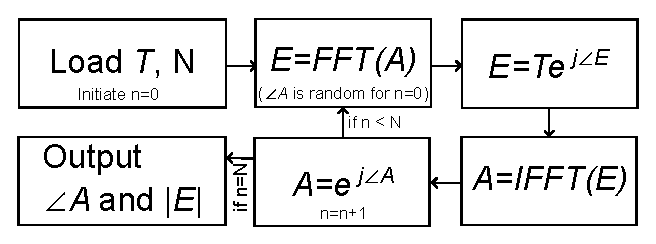
\includegraphics[width = 0.6\textwidth]{GS_flowchart.eps}
	   \end{center}
	   \caption{\label{fig:GS_flowchart} Gerchberg-Saxton (GS) algorithm flowchart}
	\end{figure}

	Then, as illustrated in \cref{fig:Quantisation_bit_depth}, a quantisation function ($Q$) can be defined by finding the closest point from one of the $2^d$ quantisation levels, given the phase ($\angle A$) and the quantisation bit depth $d$ as input.

	\begin{figure} [H]
		\begin{center}
			\begin{tabular}{c c c c}
				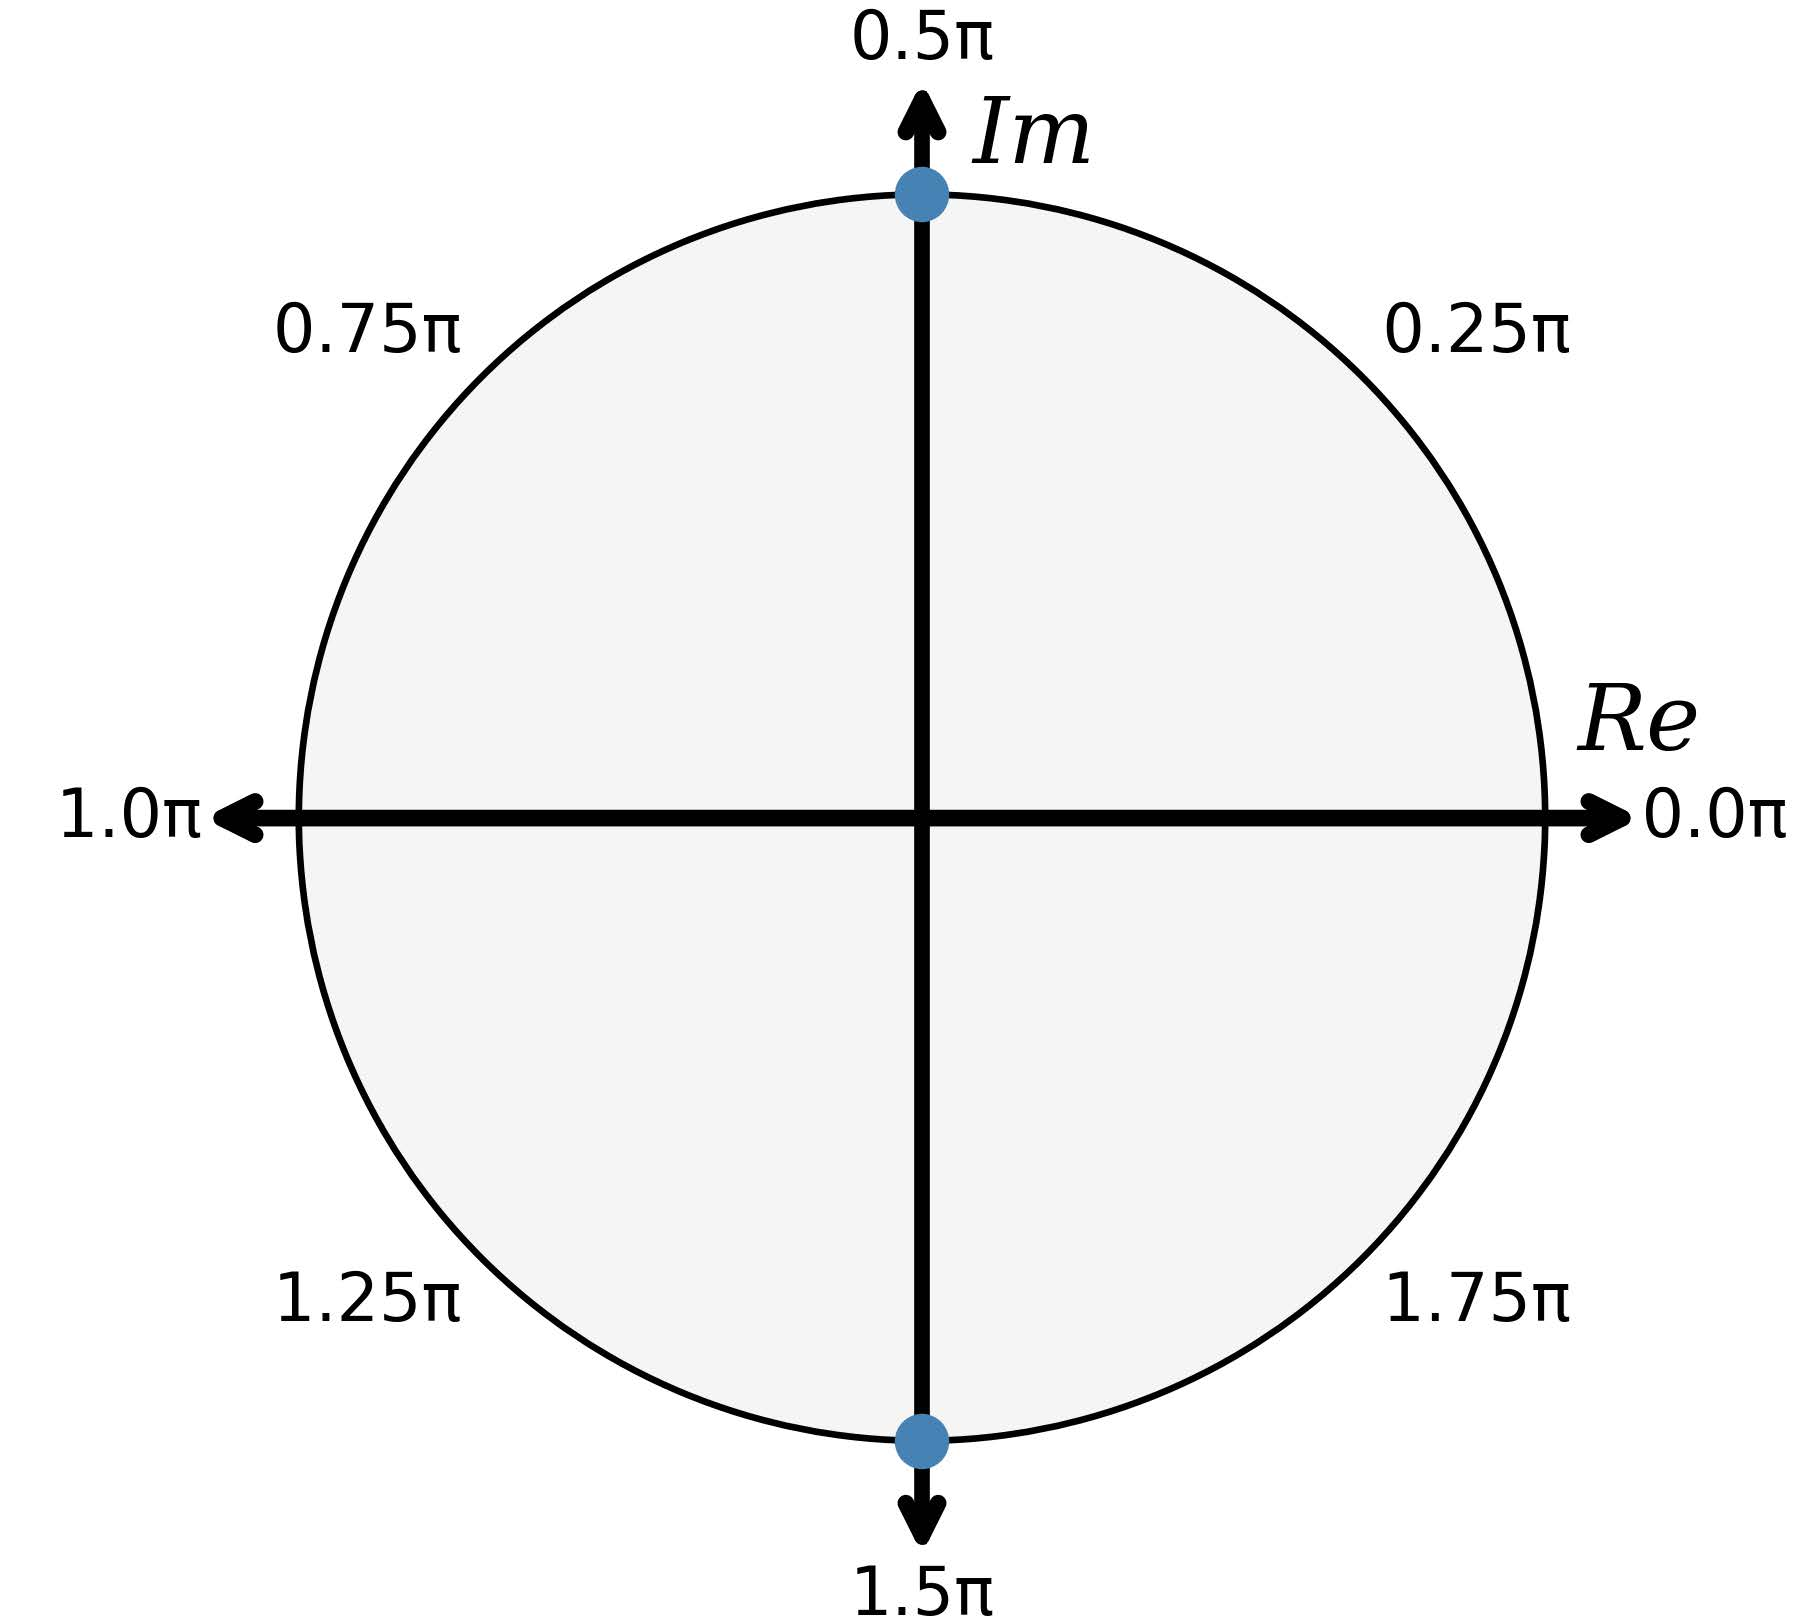
\includegraphics[width = 0.24\textwidth]{Quantization_bit_depth_1.jpg} & 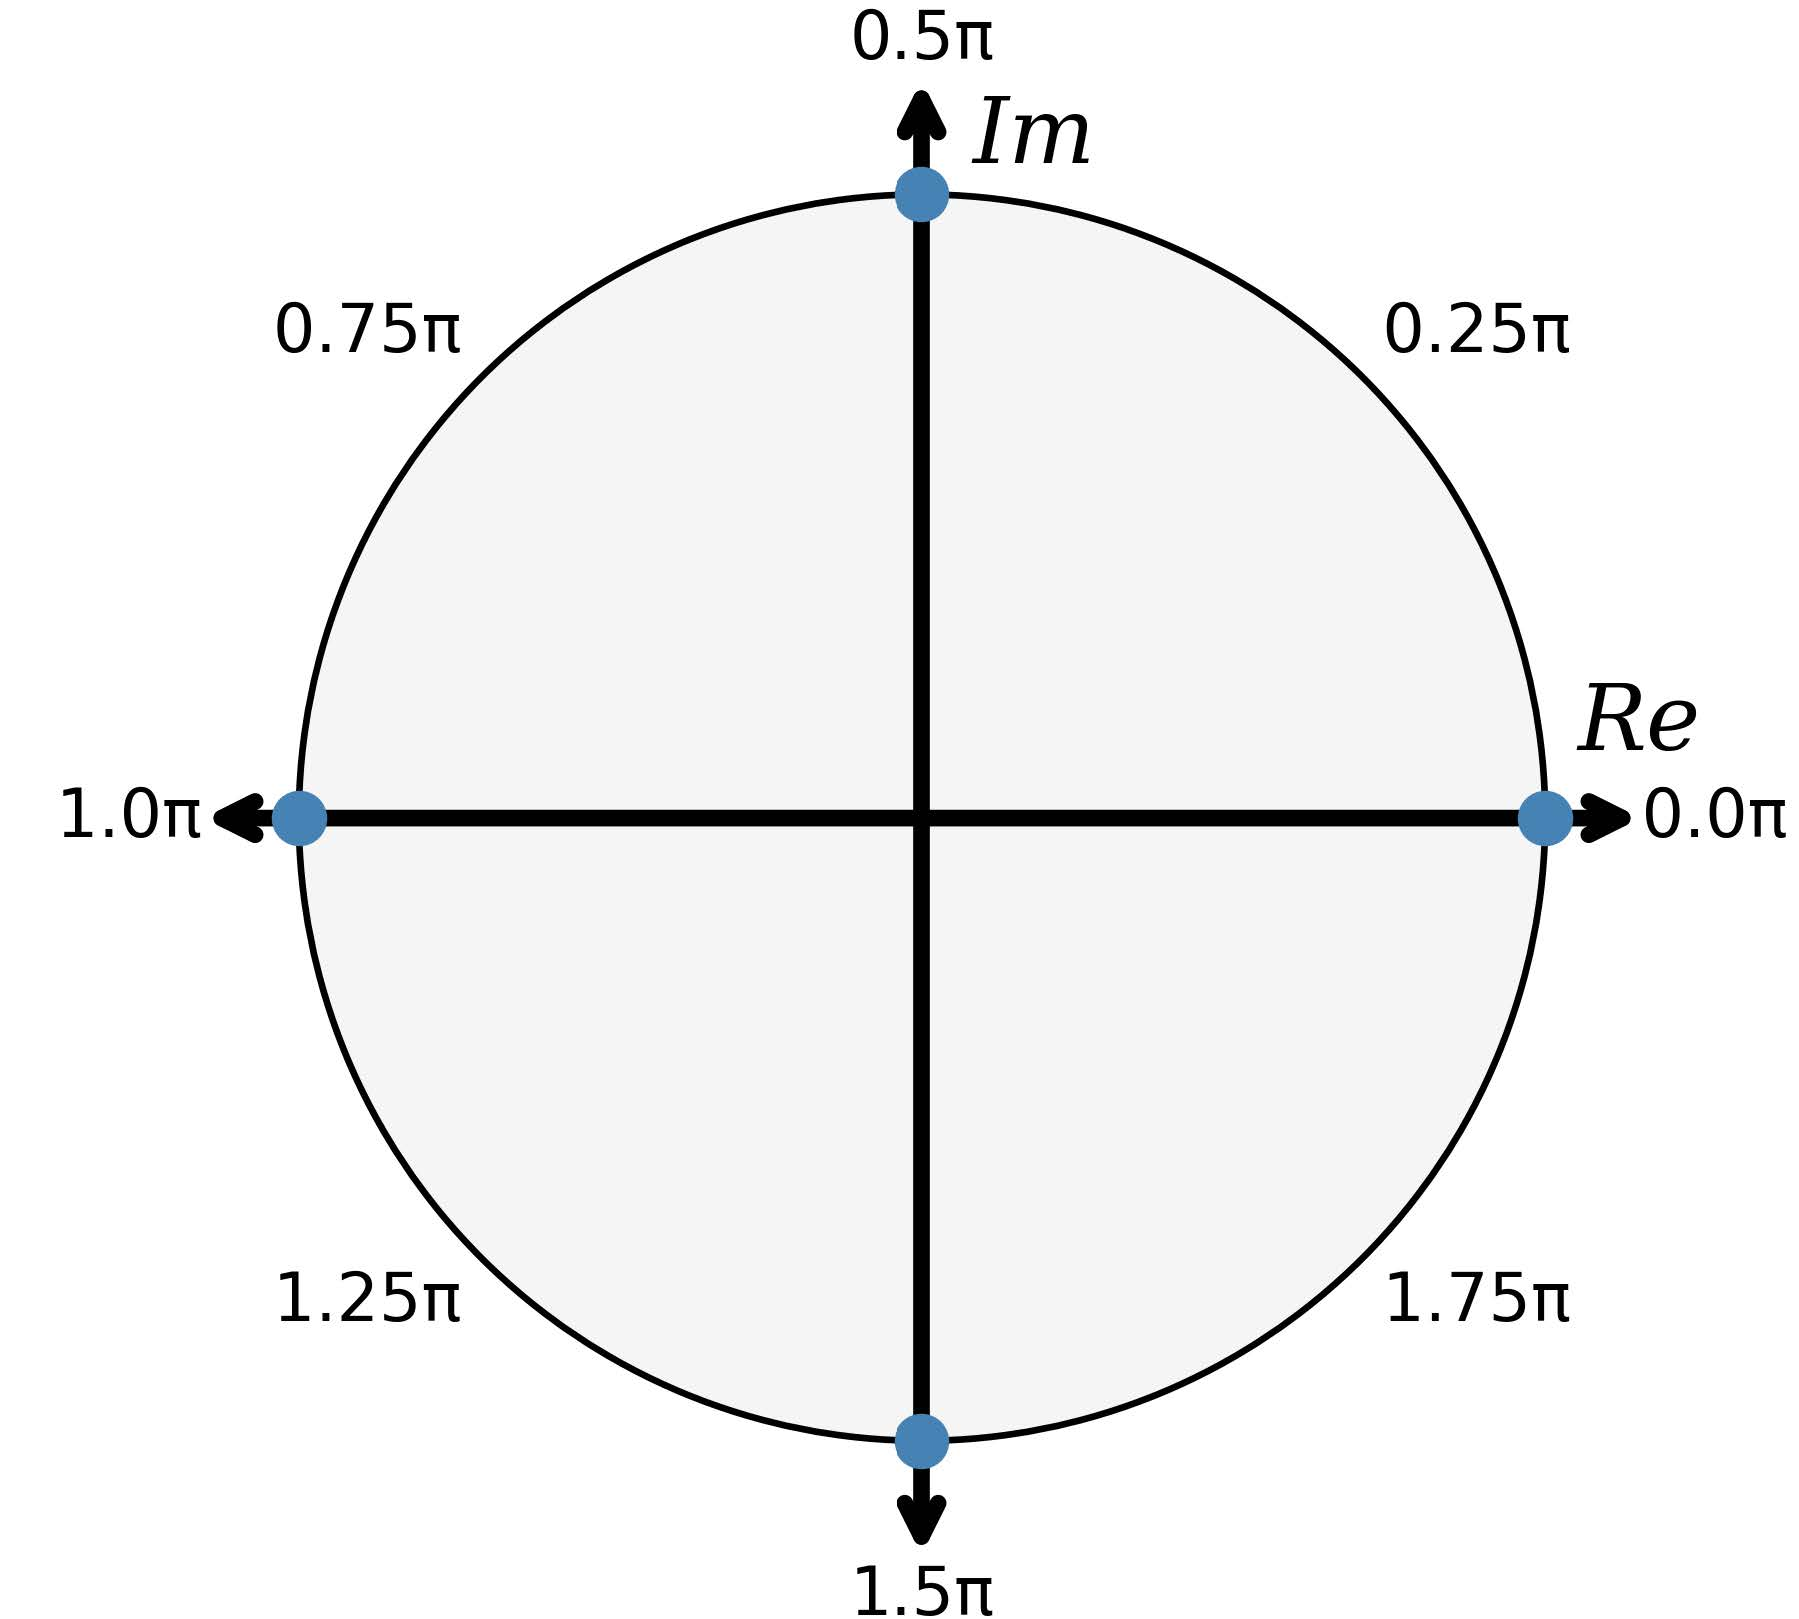
\includegraphics[width = 0.24\textwidth]{Quantization_bit_depth_2.jpg} & 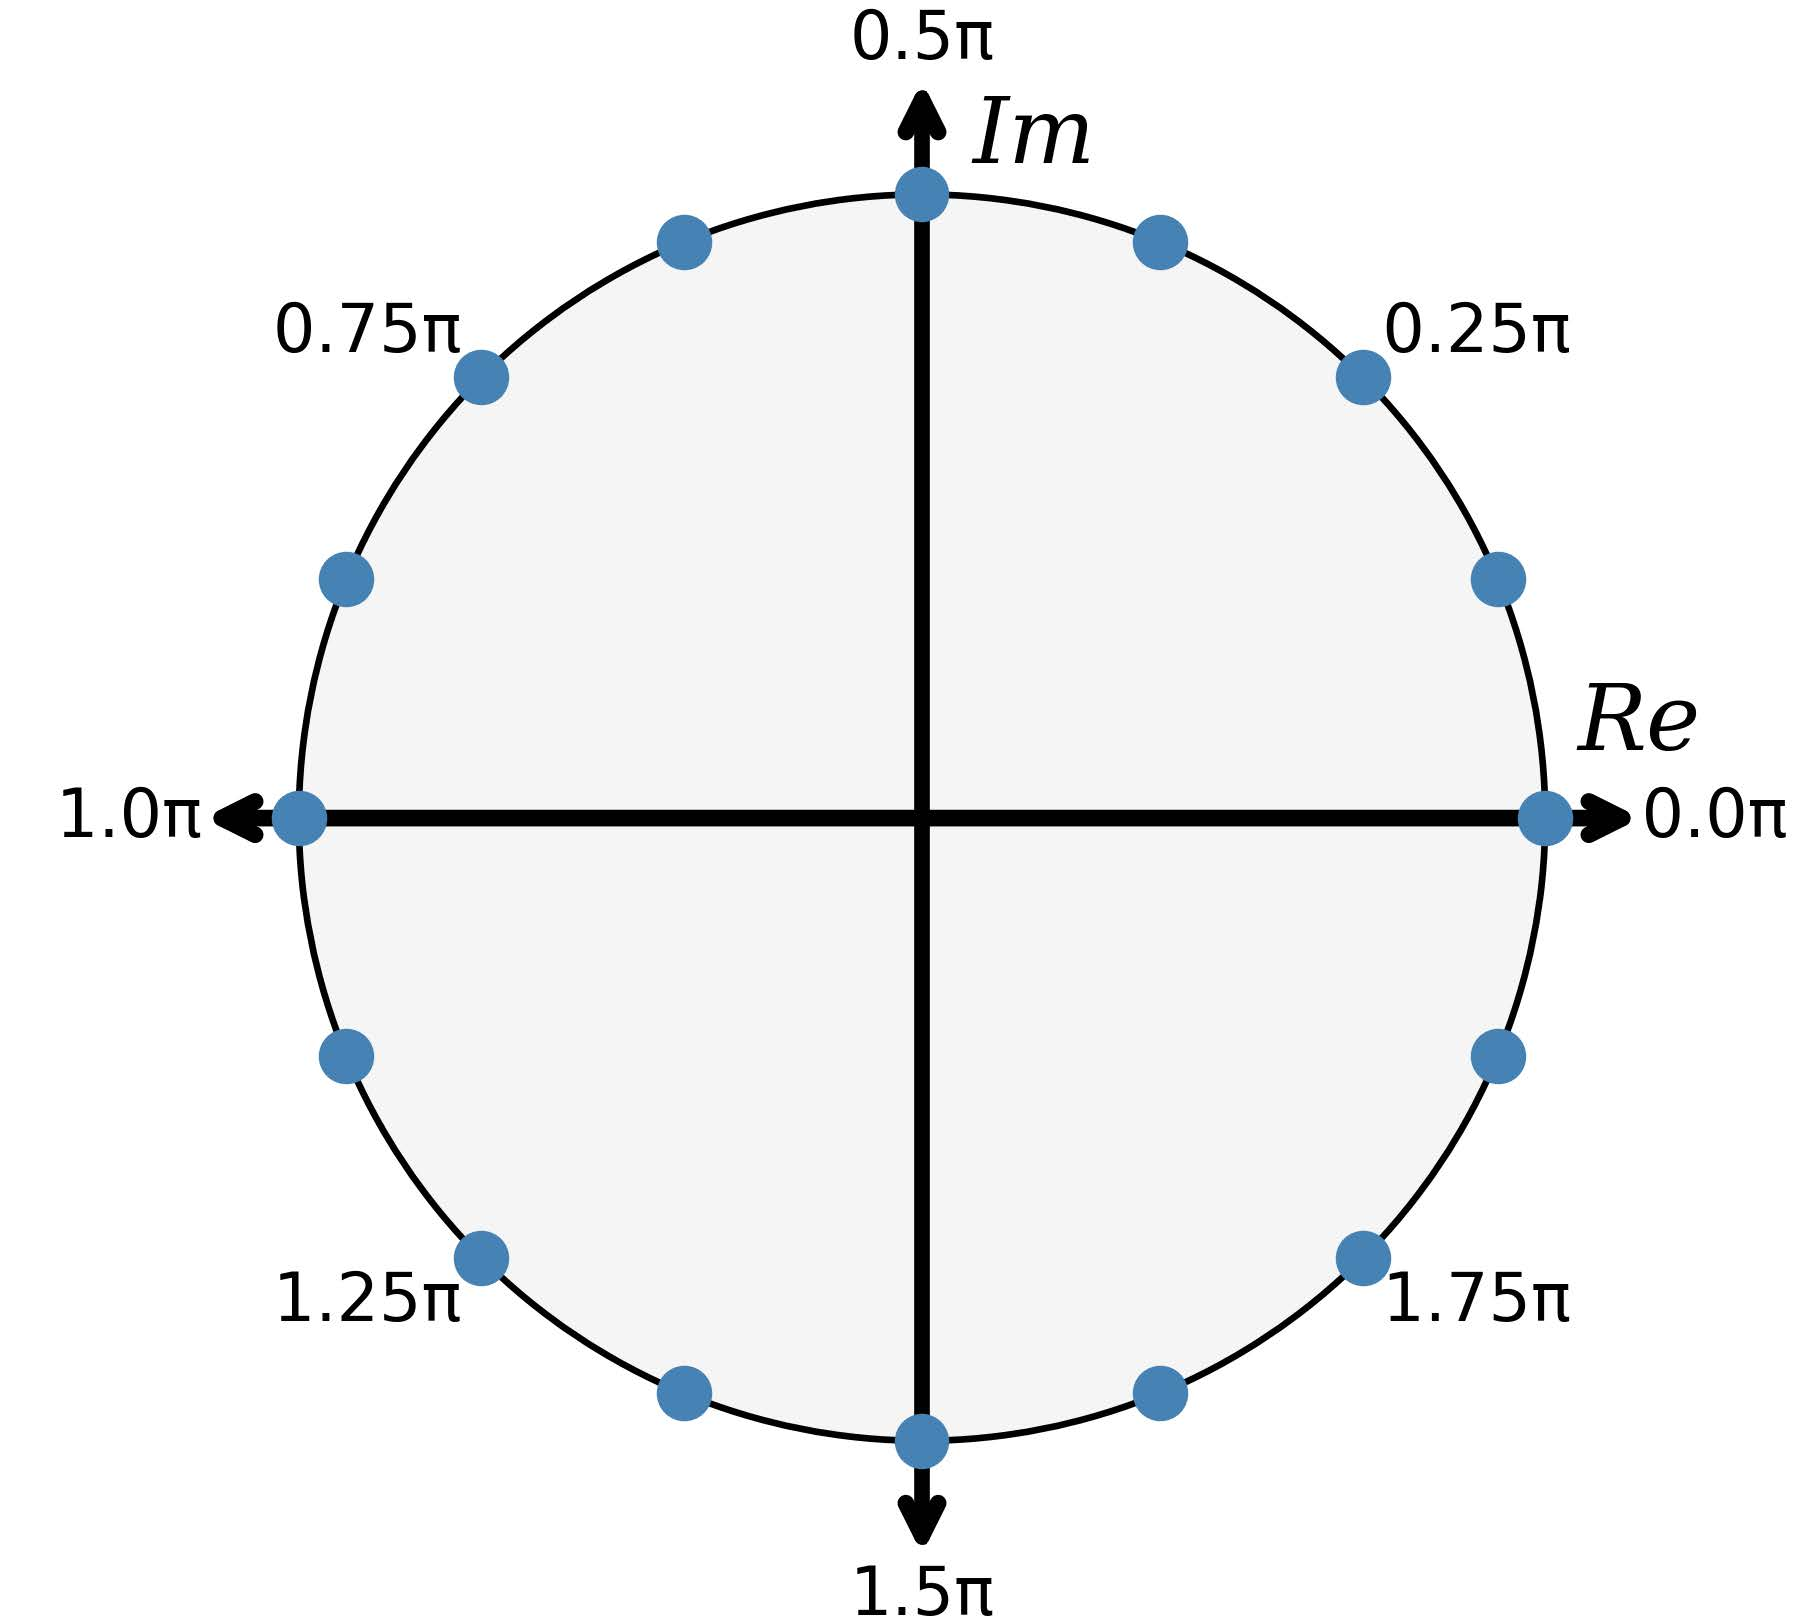
\includegraphics[width = 0.24\textwidth]{Quantization_bit_depth_4.jpg} & 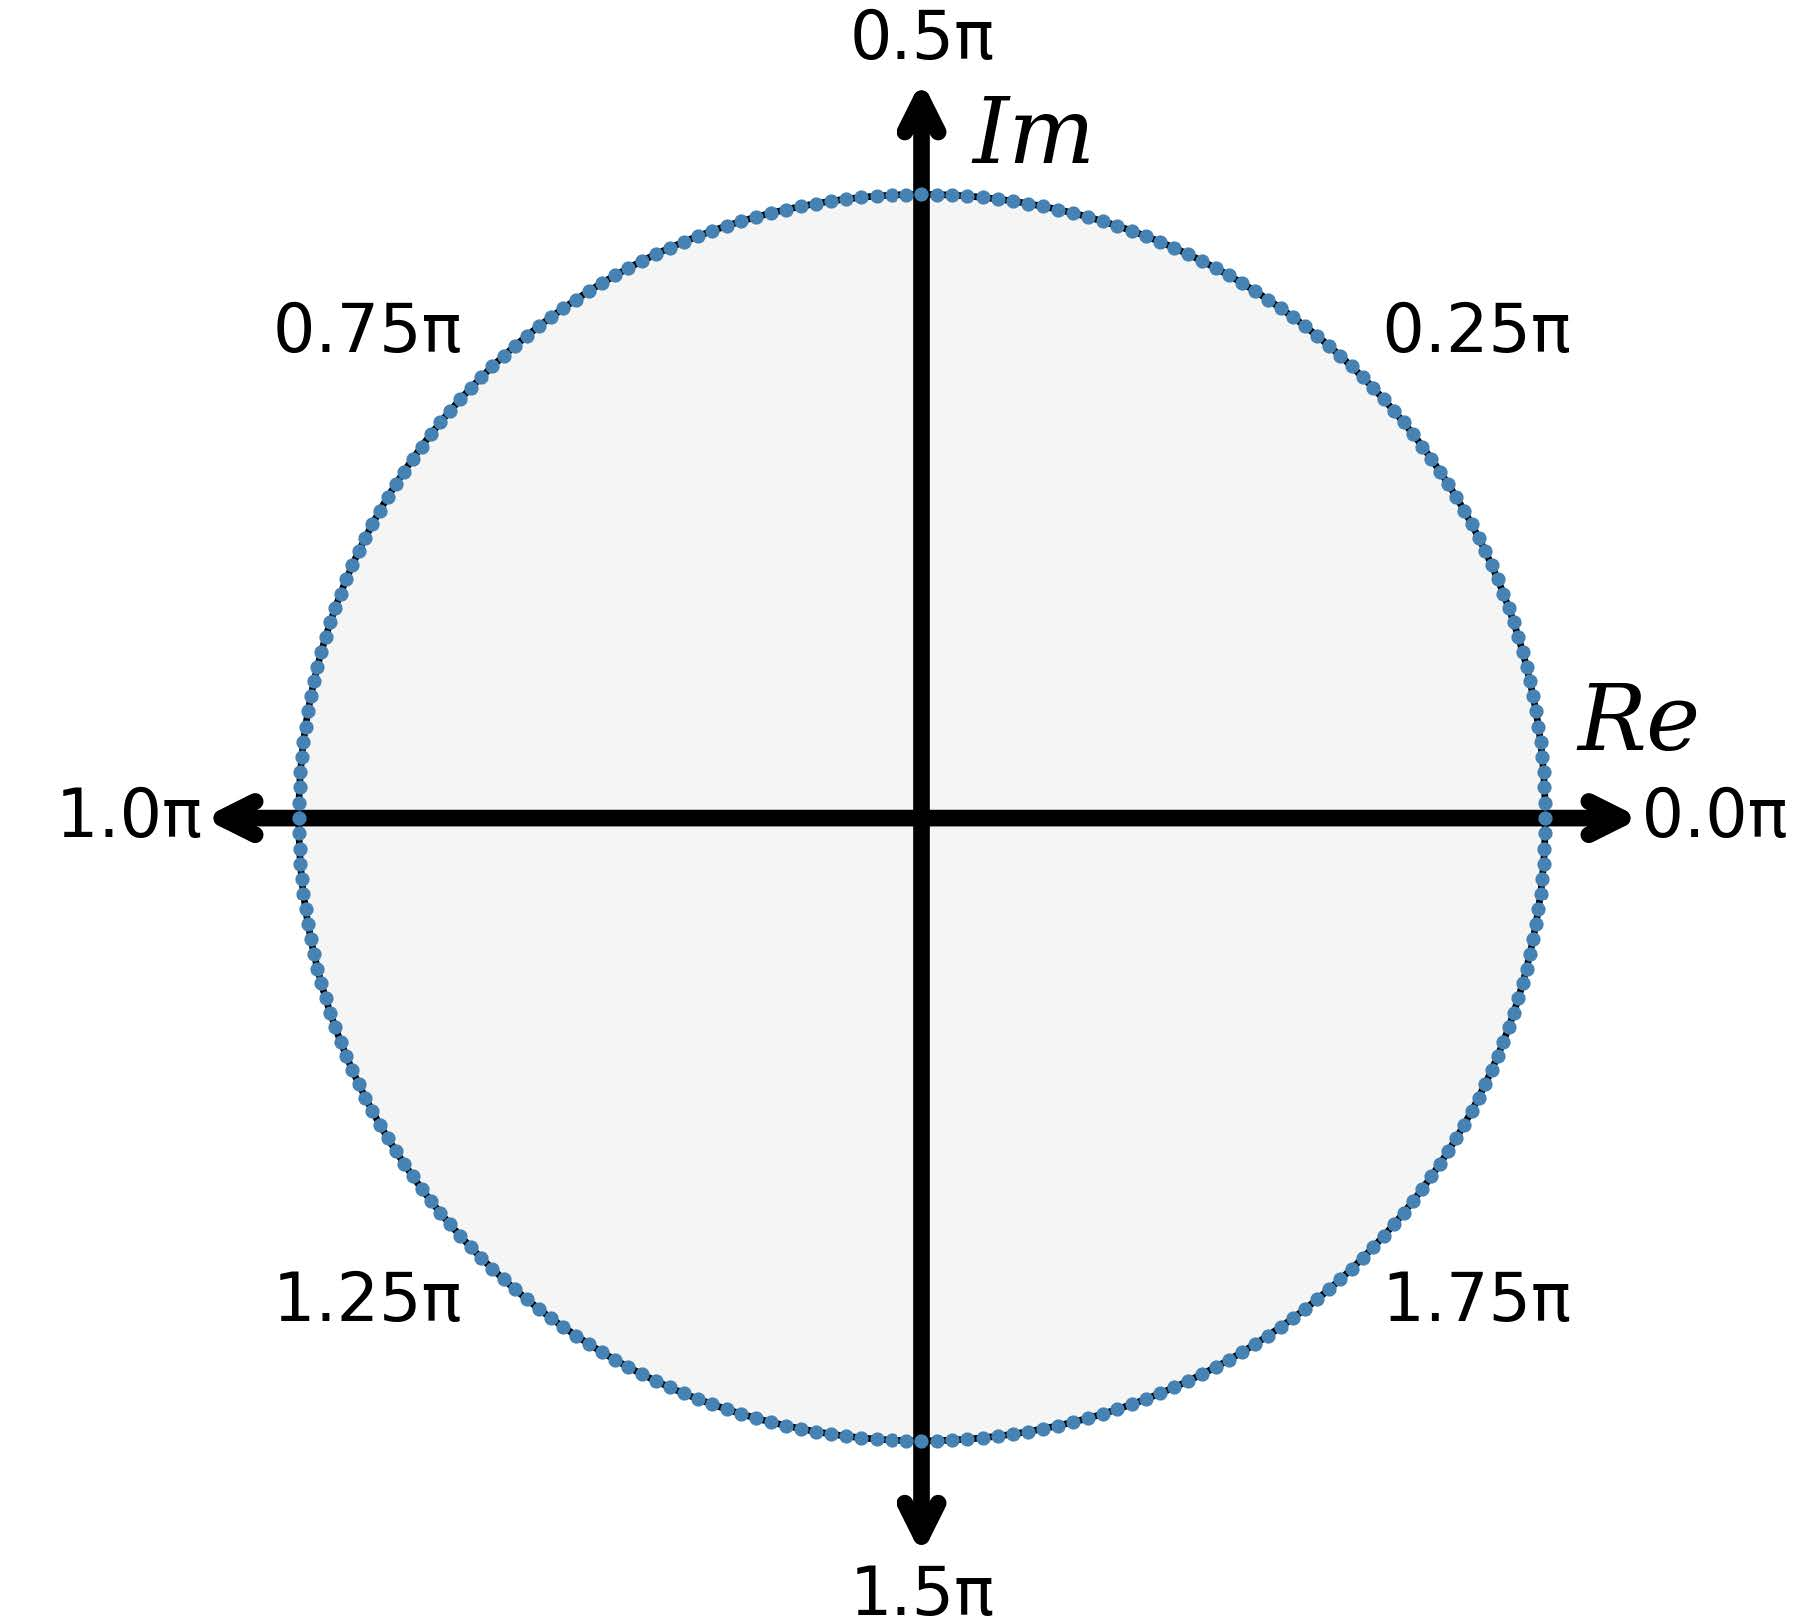
\includegraphics[width = 0.24\textwidth]{Quantization_bit_depth_8.jpg}\\
				(a) bit depth = 1 & (b) bit depth = 2 & (c) bit depth = 4 & (d) bit depth = 8
			\end{tabular}
			\caption{\label{fig:Quantisation_bit_depth} Quantisation of phase holograms}
		\end{center}
	\end{figure}

	\begin{figure} [H]
	   \begin{center}
	   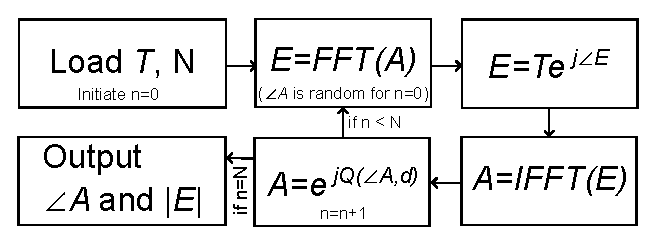
\includegraphics[width = 0.6\textwidth]{GS_quantized_flowchart.eps}
	   \end{center}
	   \caption{\label{fig:GS_quantised_flowchart} Quantised Gerchberg-Saxton (GS) algorithm flowchart}
	\end{figure}

	To compute phase holograms quantised to certain bit depth ($d$), the GS algorithm is modified to include an additional quantisation operation ($Q$) when applying the 'phase-only' constraint as shown in \cref{fig:GS_quantised_flowchart}. Such a method is better than applying the quantisation at the end of the loop, as it includes the quantisation constraint throughout the iterations, instead of introducing significant quantisation noise in the end.



\subsection{Measurement of Information}
\subsubsection{Shannon entropy}
	To quantify the information content, the classical one-dimensional (1D) Shannon entropy \cite{Shannon1948} with equation shown in \cref{eq:shannon-entropy} is selected.

	\begin{equation}
		H(X) = -\sum_{x\in X} p(x)\log_2p(x)
		\label{eq:shannon-entropy}
	\end{equation}

	Although the Shannon entropy was designed for 1D data, it can also be implemented to two-dimensional (2D) data by ignoring the 2D spatial correlations and summing $p(x)\log_2p(x)$ over the histogram of the 2D data. As only discrete data can have a meaningful Shannon entropy, the entropy can only be calculated for quantised holograms and target images, which are usually quantised to less than 8 bit depth.


\subsubsection{Delentropy} \label{sec:Delentropy}
	To account for 2D spatial correlation, the delentropy \cite{Larkin2016} is also used. Delentropy is an extension of the 1D Shannon entropy that it first computes the gradient (del) vector field image, whose entropy is then named as the delentropy, so that the spatial image structure and pixel co-occurrence can be captured \cite{Larkin2016}.

	\begin{figure} [H]
	   \begin{center}
	   \includegraphics[width = 0.8\textwidth]{delentropy.eps}
	   \end{center}
	   \caption{\label{fig:delentropy} Del operation on a sample image}
	\end{figure}

	As an example, the sample image in \cref{fig:delentropy}~(a) is the file of filename `0500.png' under the `DIV2K\_train\_HR' folder sourced from the DIV2K dataset \cite{Agustsson2017}. The sample image is calculated to have a Shannon entropy of 7.502 bits/pixel.

	\begin{equation}
		H_{PGS}(f_x, f_y) \leq \frac{H(f_x) + H(f_y)}{2}
		\label{eq:delentropy}
	\end{equation}

	By taking the $x$-derivative ($f_x$) and $y$-derivative ($f_y$) as shown in \cref{fig:delentropy}~(b)~and~(c), and using the Papoulis Generalized Sampling (PGS) \cite{Papoulis1977} theory, the delentropy is calculated using \cref{eq:delentropy}\cite{Larkin2016} to be 5.867 bits/pixel.




\section{Results}
\subsection{Targets in the far field (Fraunhofer region)} \label{sec:Fraunhofer_results}
	In this subsection, the target images are set in the far field, so the Fraunhofer diffraction formula in \cref{eq:fraunhofer-diffraction} is used.

	\begin{figure} [H]
	   \begin{center}
	   \includegraphics[width = 1.0\textwidth]{holo_bit_depth_recon_Fraunhofer.pdf}
	   \end{center}
	   \caption{\label{fig:holo_bit_depth_recon_Fraunhofer} Holograms generated at bit depths level from 1 to 8 and their according reconstructions in the far field}
	\end{figure}

	An example run of the quantised GS algorithm (in \cref{fig:GS_quantised_flowchart}) for the sample image in \cref{fig:delentropy}~(a) is shown in \cref{fig:holo_bit_depth_recon_Fraunhofer}, which demonstrates qualitatively how the reconstruction quality improves with the increase in the bit depth of the hologram, and also quantitatively as the NMSE between the reconstruction and target image has shown a decreasing trend as the bit depth of hologram increases. The rotational symmetry in the reconstruction of the hologram with bit depth 1 is explained by the conjugate properties of Fourier Transforms in \cref{sec:Rotational symmetries in the binary phase modulation}.

	Then the same quantised GS algorithm is run on the 800 images in the `DIV2K\_train\_HR' folder in the DIV2K dataset \cite{Agustsson2017}, for hologram bit depth set to integers ranging from 1 to 8, with the total number of iterations ($N$) set to 100.

	\begin{figure} [H]
	   \begin{center}
	   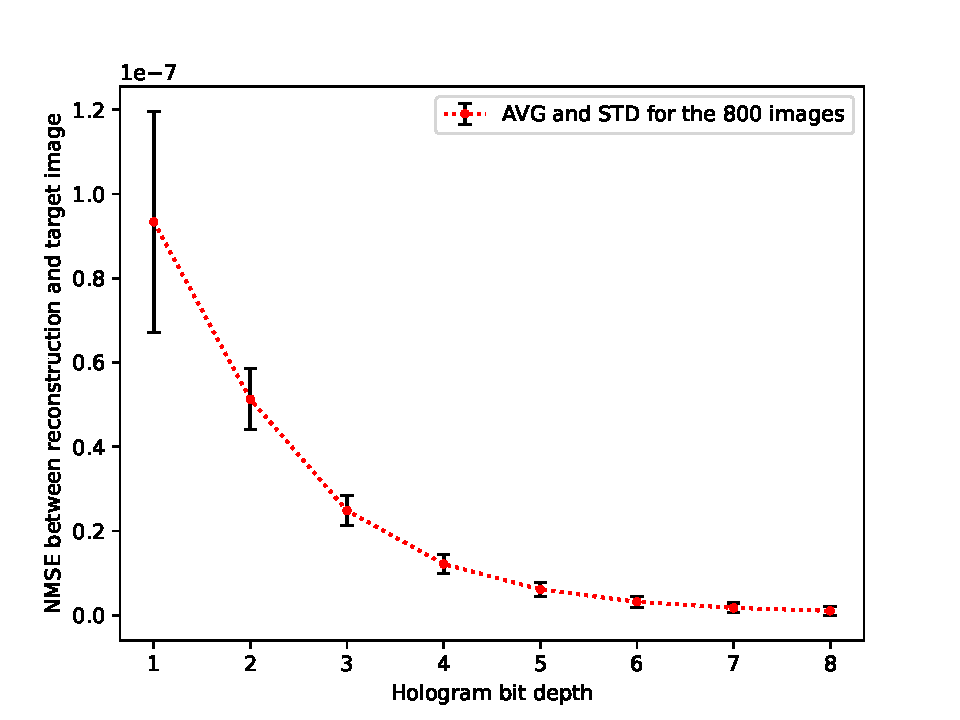
\includegraphics[width = \textwidth]{GS_Fraunhofer_NMSE_VS_Hologram bit depth.pdf}
	   \end{center}
	   \caption{\label{fig:GS_Fraunhofer_NMSE_VS_Hologram_bit_depth} The average and standard deviation of the far-field reconstruction errors among the 800 target images plotted against the hologram bit depth}
	\end{figure}

	For the 800 target images, the average (AVG) and standard deviation (STD) of the NMSE values between the far-field reconstructions of the holograms and their corresponding target images are plotted against the hologram bit depth in \cref{fig:GS_Fraunhofer_NMSE_VS_Hologram_bit_depth} (the raw data is accessible from the published research dataset \cite{research_data_Sha2024}). It can be concluded that, the NMSE between the resulting reconstructions and their according target images decreases as the hologram bit depth increases. As holograms with higher bit depths can carry more information according to the information theory, they are more capable of storing the information needed to better reconstruct the target images.

	\begin{figure} [H]
		\begin{center}
		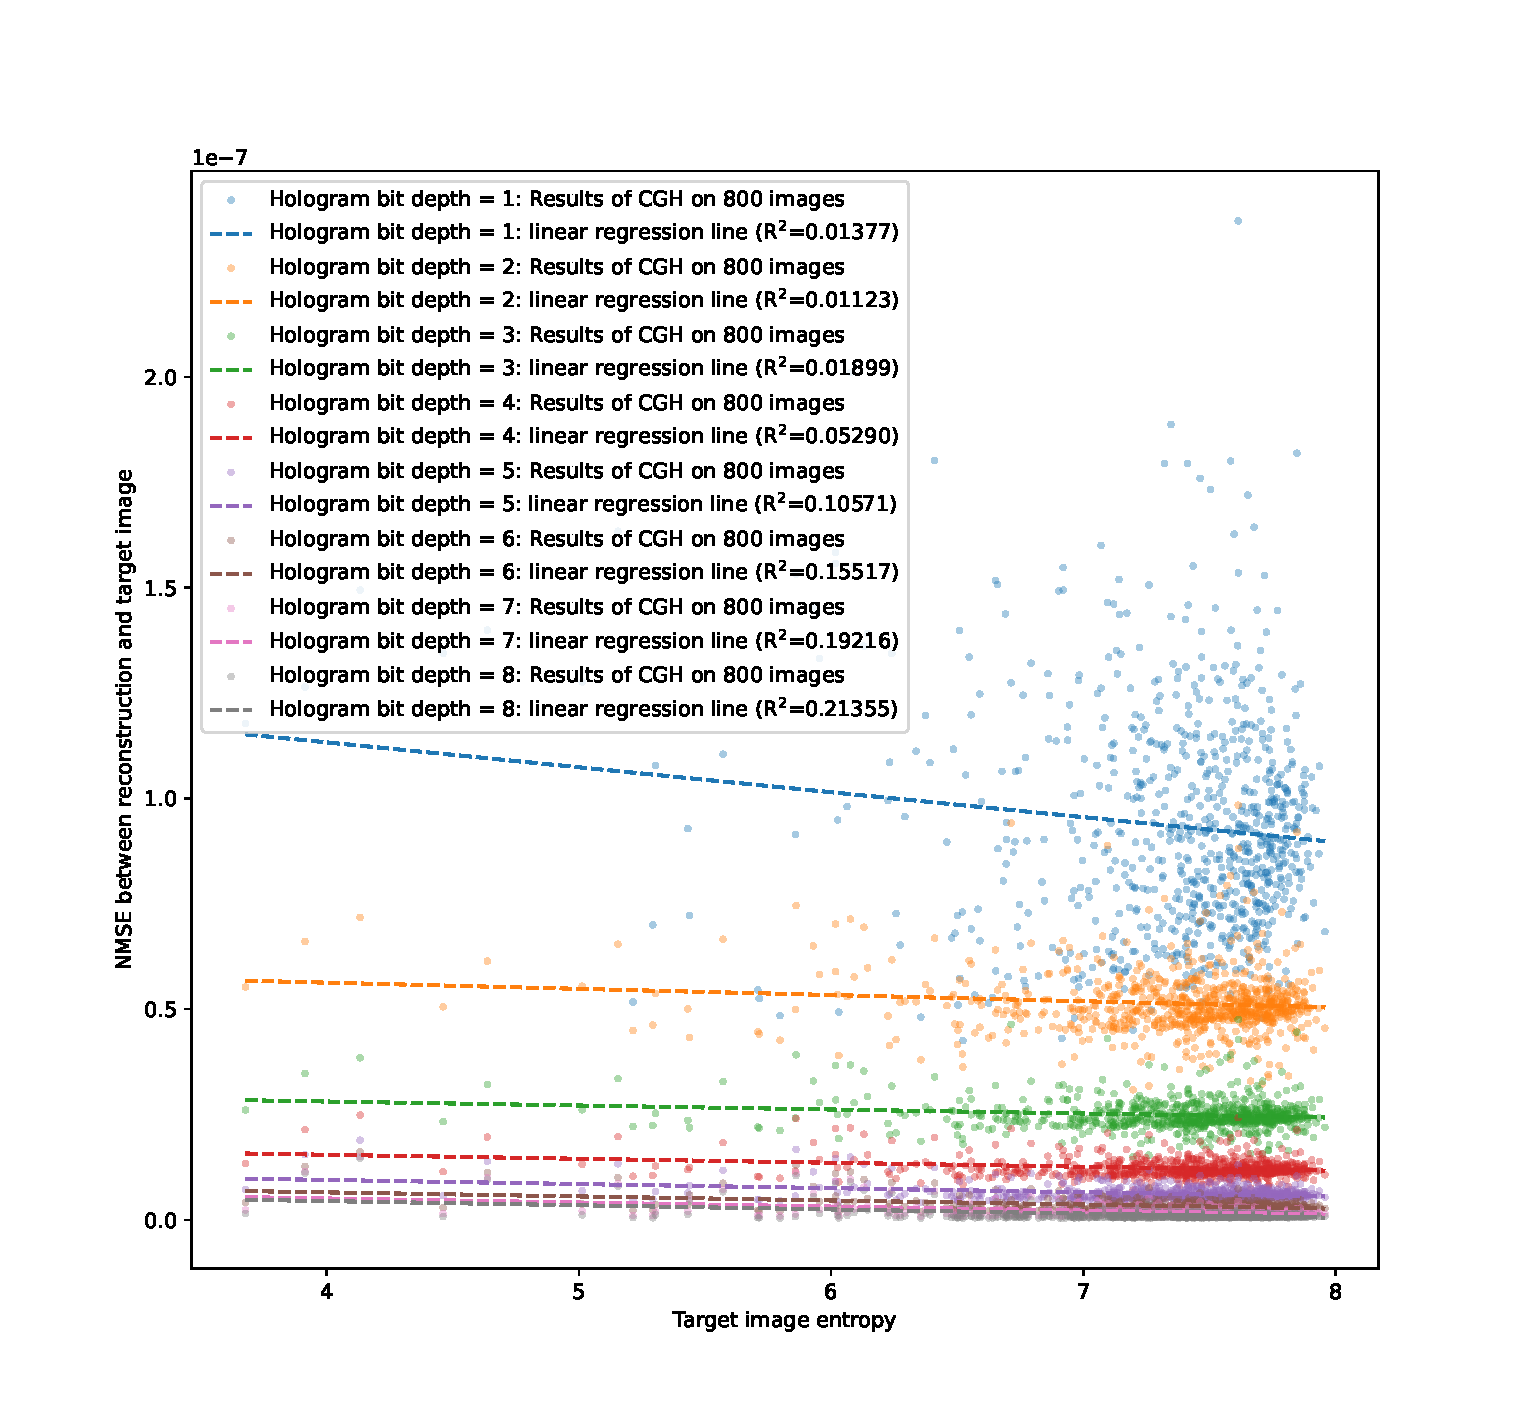
\includegraphics[trim={50 40 70 70}, clip, width = \textwidth]{GS_Fraunhofer_NMSE_VS_Entropy.pdf}
		\end{center}
		\caption{\label{fig:GS_Fraunhofer_NMSE_VS_Entropy} Scatter plot of the far-field reconstruction errors v.s. entropy of target image among the 800 target images, with different colours indicating hologram bit depth constraints}
	\end{figure}

	Then the entropy of each of the 800 target images are calculated using \cref{eq:shannon-entropy}, and a scatter plot of the NMSE between the far-field reconstruction and target image against the target image entropy is plotted for all 800 target images run with each of the 8 hologram bit depth levels, as shown in \cref{fig:GS_Fraunhofer_NMSE_VS_Entropy}. To avoid the effect of the different initial random phases on the final result, 5 different randomly generated initial phases are used for each run; however, the result \cite{research_data_Sha2024} has shown negligible difference between the runs using different random initial phase holograms.
	Unfortunately, as the linear regressions between NMSE and entropies of target image have coefficients of determination ($R^2$) much less than 0.5, no correlation has been found between the NMSE and the target image entropy. Therefore, the Shannon entropy cannot be used to quantify the difficulty of CGH for a given target image.


	\begin{figure} [H]
		\begin{center}
		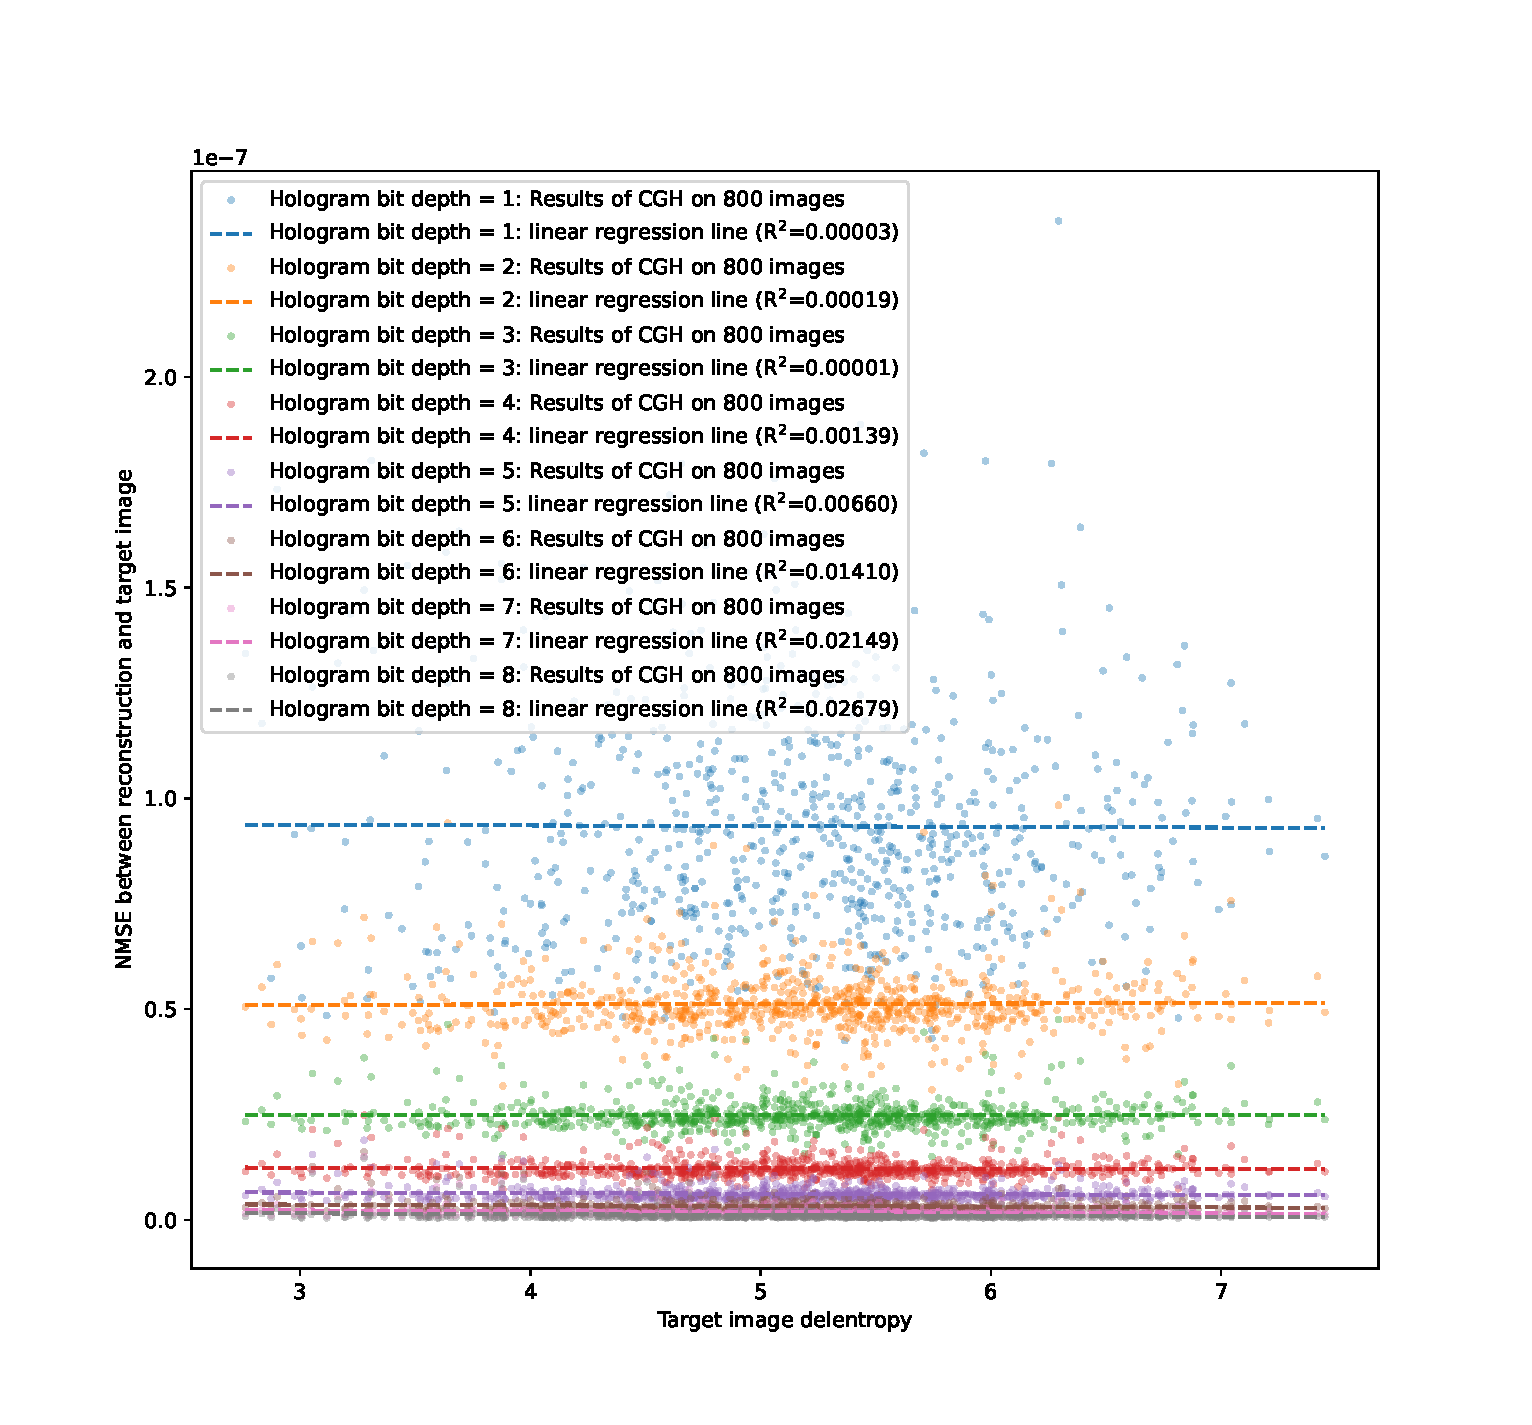
\includegraphics[trim={50 40 70 70}, clip, width = \textwidth]{GS_Fraunhofer_NMSE_VS_Delentropy.pdf}
		\end{center}
		\caption{\label{fig:GS_Fraunhofer_NMSE_VS_Delentropy} Scatter plot of the far-field reconstruction errors v.s. delentropy of target image among the 800 target images, with different colours indicating hologram bit depth constraints}
	\end{figure}

	The delentropy of each of the 800 target images are then calculated using the method in \cref{sec:Delentropy}, and a scatter plot of the NMSE between the far-field reconstruction and target image against the target image delentropy is plotted in \cref{fig:GS_Fraunhofer_NMSE_VS_Delentropy} for the 800 target images. And again, as all the $R^2$ are much less than 0.5, no correlation is shown between the NMSE and the target image delentropy, inferring that the 2D delentropy also fails to predict the error of CGH for a given target image.


\subsection{Targets in the near field (Fresnel region)}
	The target images are now set to near field, where the Fresnel diffraction formula in \cref{eq:fresnel-diffraction} applies; therefore the FFT and IFFT stages in \cref{fig:GS_quantised_flowchart} are modified to include the phase term in \cref{eq:fresnel-diffraction}, and for experimental purpose, the distance ($z$) is set at $10cm$, the hologram's pixel pitch (sampling resolution of $x$ and $y$) has a size of $13.62\mu m$ and the incident light's wavelength ($\lambda$) is $532nm$.
	\begin{figure} [H]
	   \begin{center}
	   \includegraphics[width = 1.0\textwidth]{holo_bit_depth_recon_Fresnel.pdf}
	   \end{center}
	   \caption{\label{fig:holo_bit_depth_recon_Fresnel} Holograms generated at bit depths level from 1 to 8 and their according reconstructions in the near field}
	\end{figure}

	\cref{fig:holo_bit_depth_recon_Fresnel} shows both qualitatively and quantitatively how the reconstruction quality improves (i.e. NMSE decreases) with the increase in the bit depth of the hologram. Such a trend is the same for target images placed in the near field as those placed in the far field in \cref{fig:holo_bit_depth_recon_Fraunhofer}. The rotational symmetry is gone for the binary phase hologram (bit depth = 1) due to the extra phase term in the Fresnel diffraction formula making the product of binary phase hologram and the phase term to be complex-valued whose complex conjugate does not equal to itself; however, the complex conjugate wouldn't disappear, but it will appear at a different distance to where the target image is set at, leading to extra defocused noise onto the reconstruction plane. Nevertheless, the trend of NMSE shows that holograms with higher bit depth produces better quality in the reconstruction plane.

	\begin{figure} [H]
	   \begin{center}
	   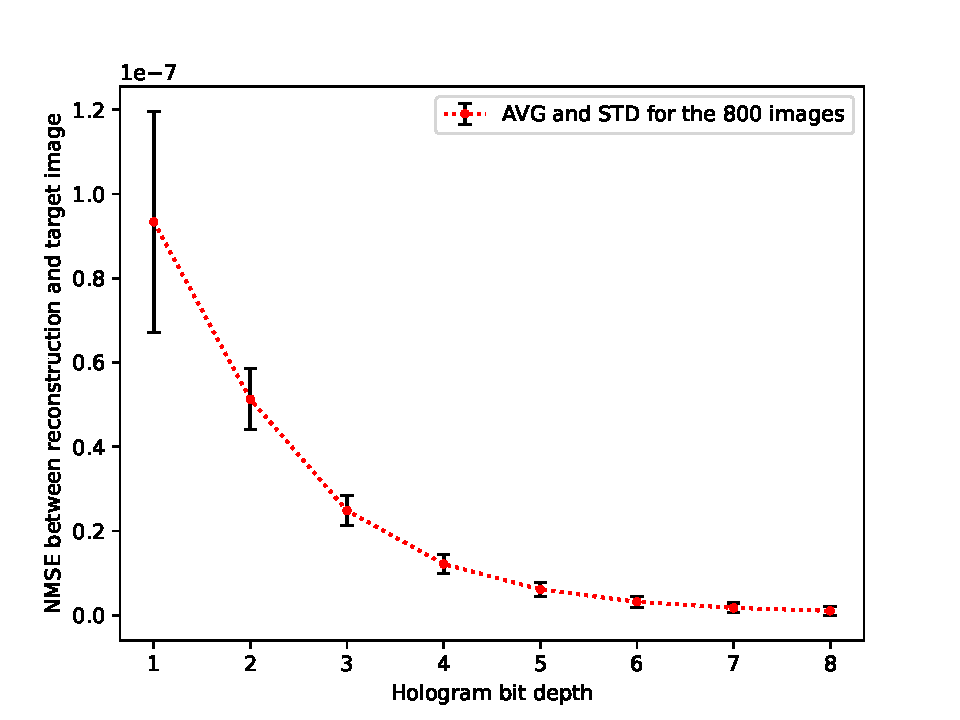
\includegraphics[width = \textwidth]{GS_Fraunhofer_NMSE_VS_Hologram bit depth.pdf}
	   \end{center}
	   \caption{\label{fig:GS_Fresnel0.1_NMSE_VS_Hologram_bit_depth} The average and standard deviation of the near-field reconstruction errors among the 800 target images plotted against the hologram bit depth}
	\end{figure}

	\cref{fig:GS_Fresnel0.1_NMSE_VS_Hologram_bit_depth} plots the average (AVG) and standard deviation (STD) of the NMSE values between the near-field reconstructions of the holograms and their corresponding target images against the hologram bit depth (the raw data is accessible from the published research dataset \cite{research_data_Sha2024}). In \cref{fig:GS_Fresnel0.1_NMSE_VS_Hologram_bit_depth}, the same trend as the one for far field in \cref{fig:GS_Fraunhofer_NMSE_VS_Hologram_bit_depth} can be observed, where NMSE decreases as hologram bit depth increases, for every single target image. Therefore, the previous conclusion of higher hologram bit depth being able to produce better reconstruction quality is still valid.


	\begin{figure} [H]
		\begin{center}
		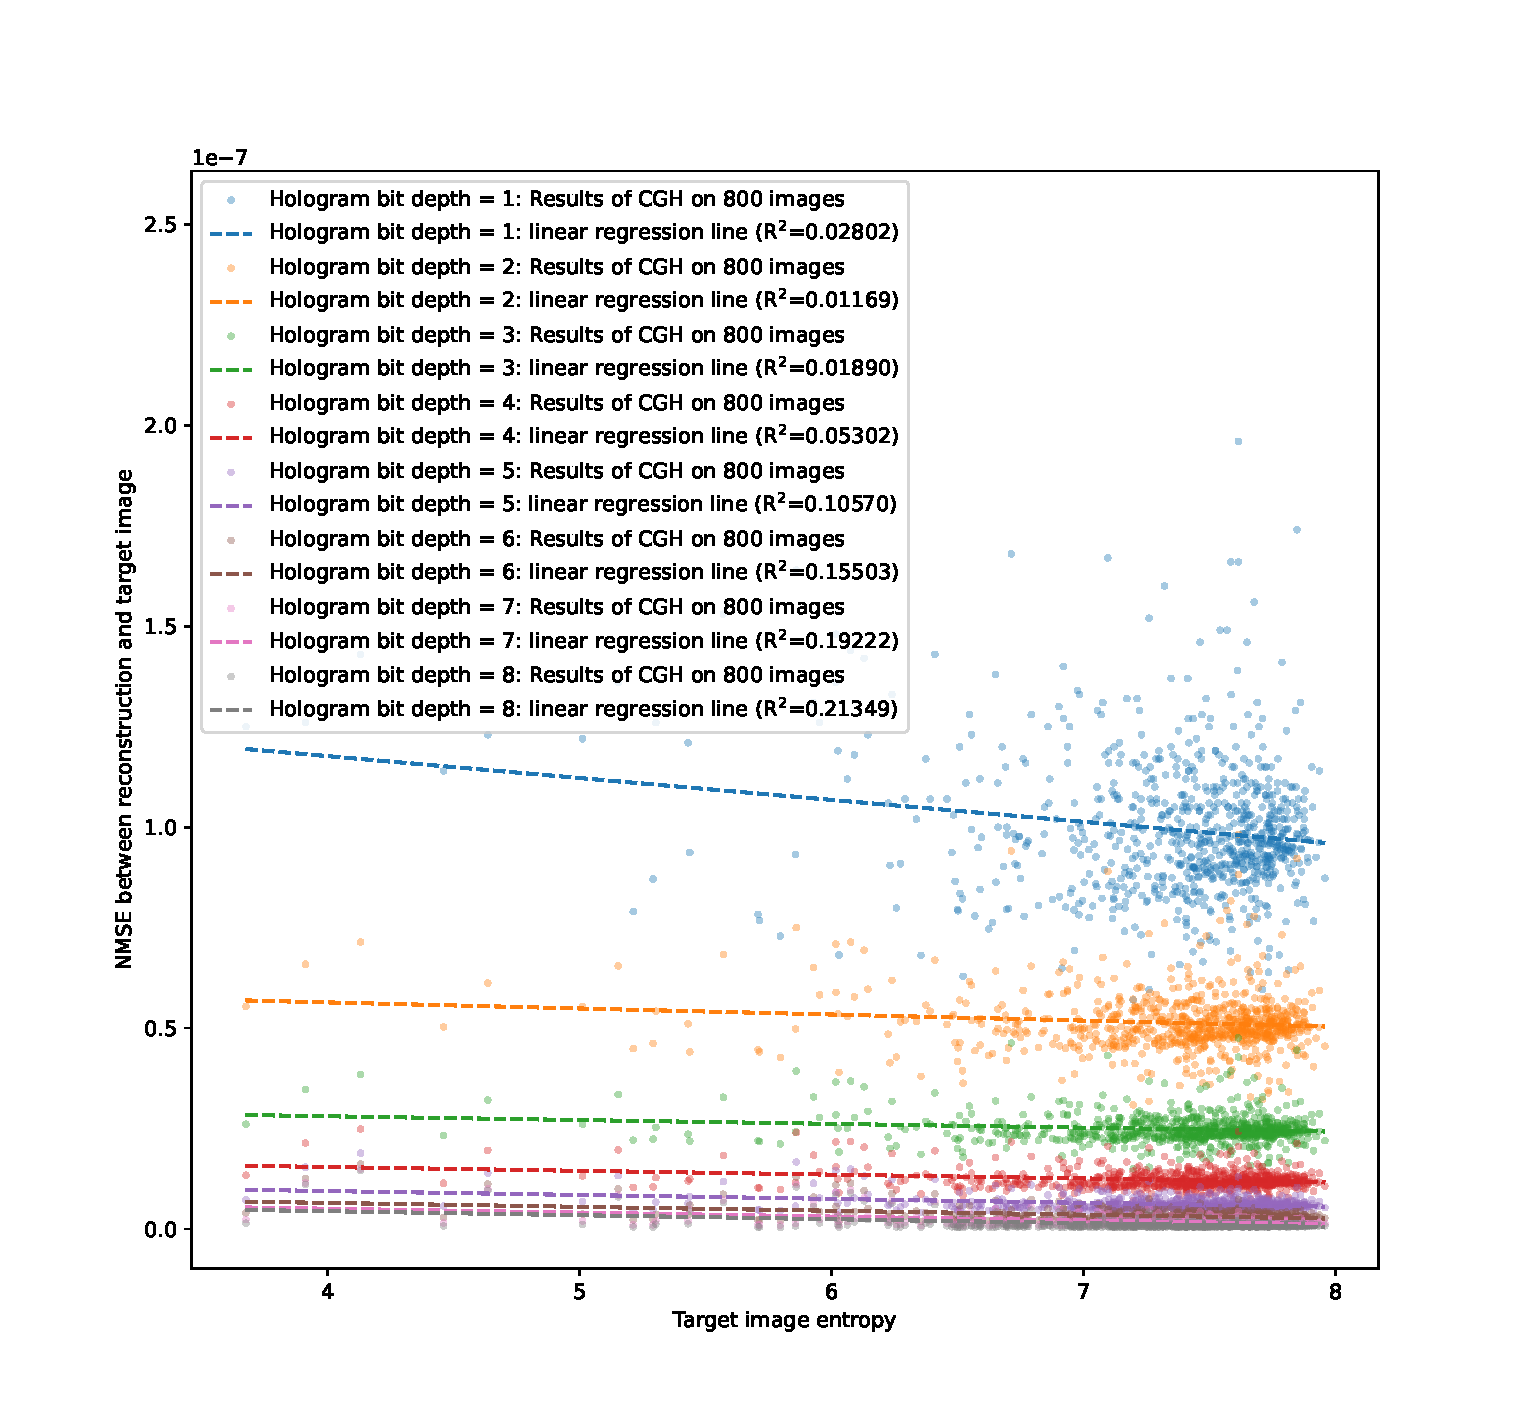
\includegraphics[trim={50 40 70 70}, clip, width = \textwidth]{GS_Fresnel0.1_NMSE_VS_Entropy.pdf}
		\end{center}
		\caption{\label{fig:GS_Fresnel0.1_NMSE_VS_Entropy} Scatter plot of the near-field reconstruction errors v.s. entropy of target image among the 800 target images, with different colours indicating hologram bit depth constraints}
	\end{figure}

	A scatter plot of the NMSE between the near-field reconstruction and target image against the target image entropy is plotted for all 800 target images run with each of the 8 hologram bit depth levels as shown in \cref{fig:GS_Fresnel0.1_NMSE_VS_Entropy}, with the hologram bit depth distinguished by different colours.
	Unfortunately, as the linear regressions between NMSE and entropies of target image have coefficients of determination ($R^2$) much less than 0.5, no correlation has been found between the NMSE and the target image entropy. Therefore, the Shannon entropy cannot be used to quantify the difficulty of CGH for a given target image.


	\begin{figure} [H]
		\begin{center}
		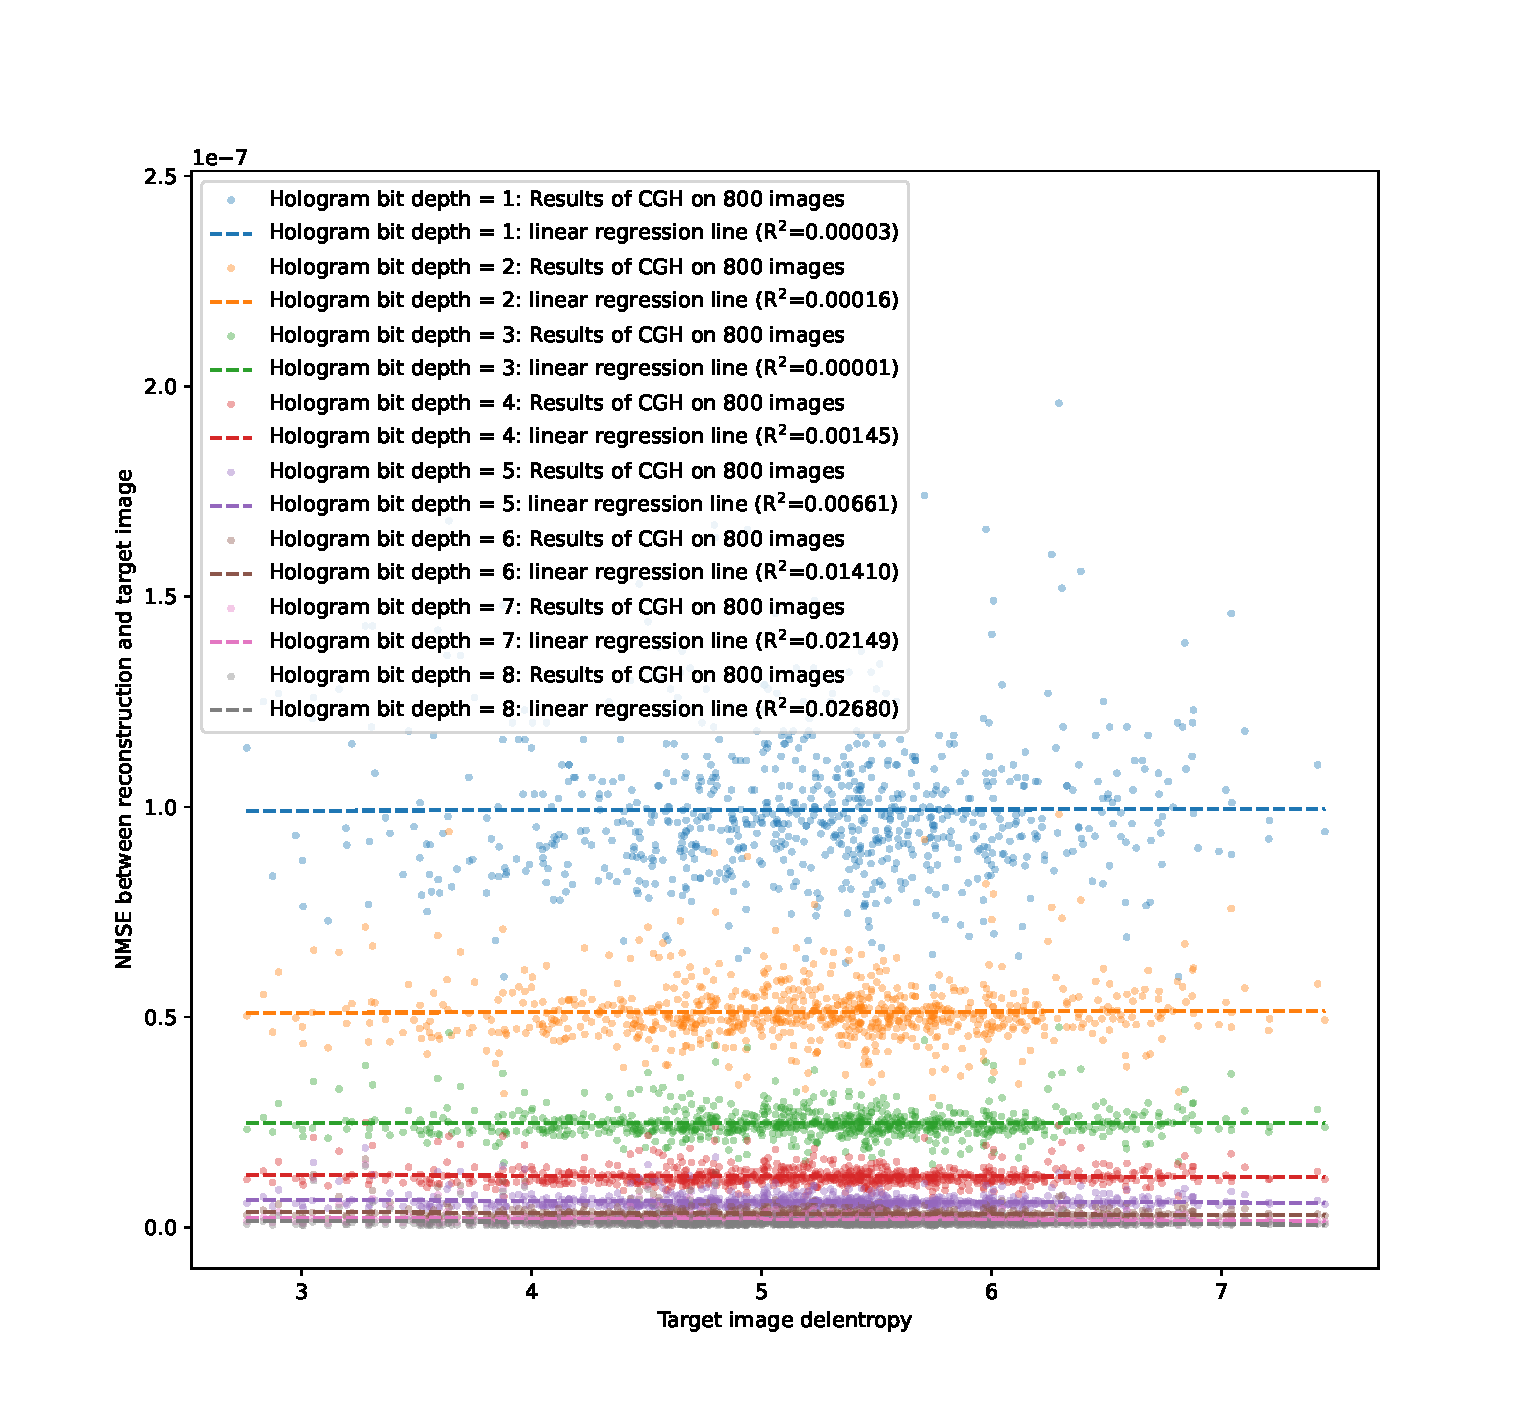
\includegraphics[trim={50 40 70 70}, clip, width = \textwidth]{GS_Fresnel0.1_NMSE_VS_Delentropy.pdf}
		\end{center}
		\caption{\label{fig:GS_Fresnel0.1_NMSE_VS_Delentropy} Scatter plot of the near-field reconstruction errors v.s. delentropy of target image among the 800 target images, with different colours indicating hologram bit depth constraints}
	\end{figure}


	The scatter plot ofthe NMSE between the near-field reconstruction and target image against the target image delentropy in \cref{fig:GS_Fresnel0.1_NMSE_VS_Delentropy} again shows no correlation between the NMSE and the delentropy of target image. Such `no correlation' result is the same as the results for far field investigated in \cref{sec:Fraunhofer_results}, confirming that neither entropy nor delentropy is suitable for quantifying how difficult a target image is for CGH.



	\begin{figure} [H]
		\begin{center}
			\begin{tabular}{c c}
				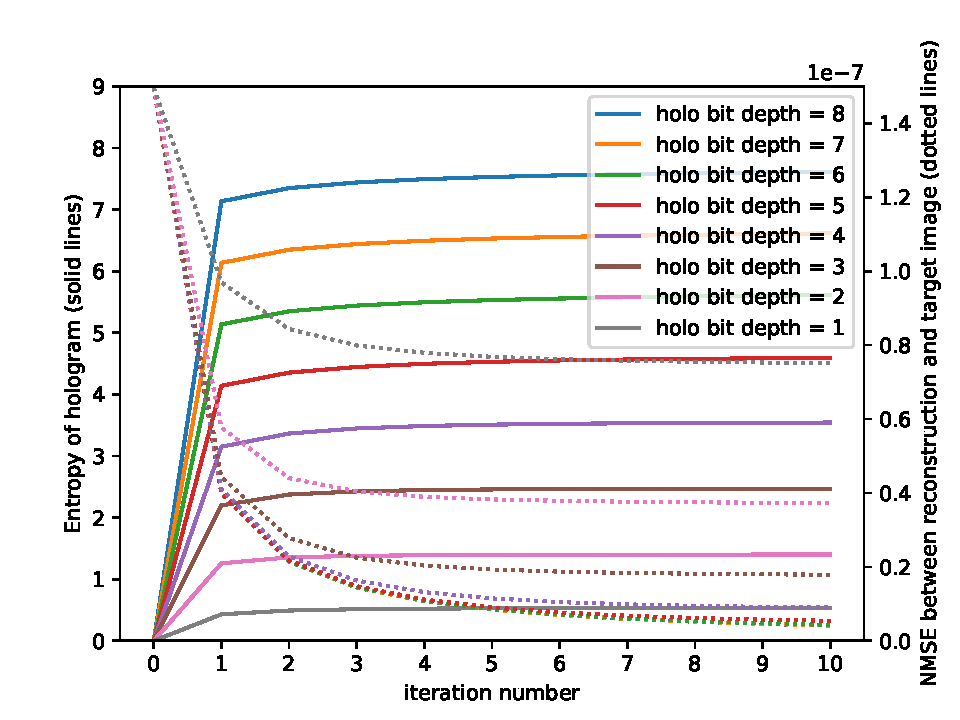
\includegraphics[trim={30 0 10 20}, clip, width = 0.9\textwidth]{GS_Fresnel0.1_iterations_zero_start.pdf}\vspace{-5mm} \\
				(a)\\ \vspace{-2mm}
				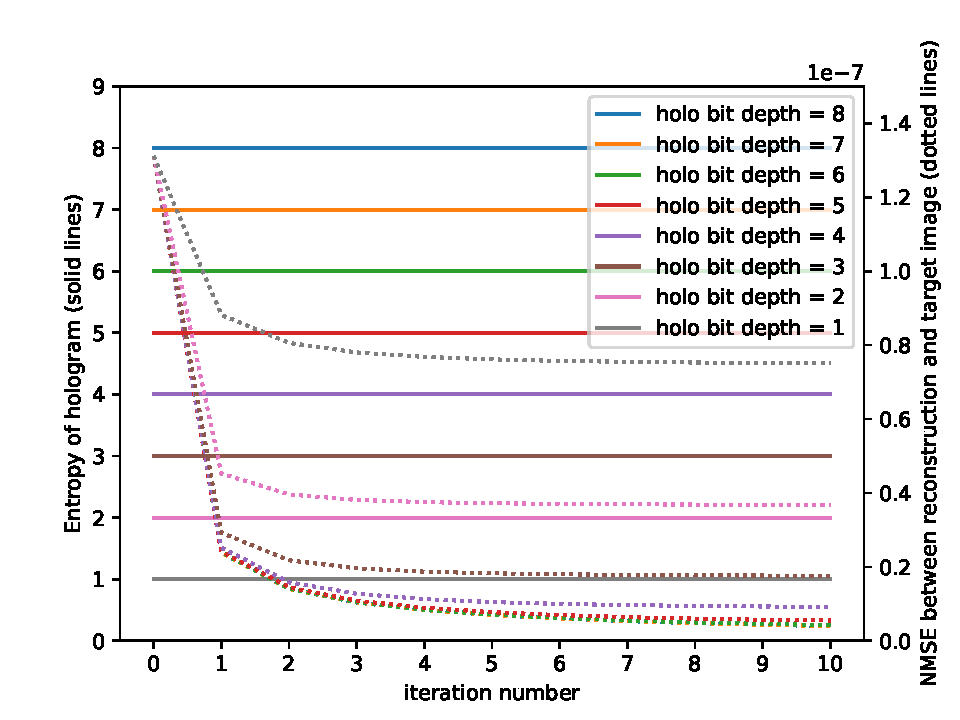
\includegraphics[trim={30 0 10 20}, clip, width = 0.9\textwidth]{GS_Fresnel0.1_iterations_random_start.pdf}\vspace{-4mm} \\
				(b) \vspace{-2mm}
			\end{tabular}
			\caption{\label{fig:GS_Fresnel0.1_iterations} Hologram entropy (solid lines) and NMSE (dotted lines) plotted against the iteration number in a GS run with the initial hologram phase ($\angle A$) being (a) zeros (b) random}
		\end{center}
	\end{figure}

	The research moves on to investigate the entropy of holograms. In an example run for a quantised hologram generation in the near field, both the hologram entropy and the NMSE between reconstruction and target image are recorded and plotted in \cref{fig:GS_Fresnel0.1_iterations}~(a)~and~(b) for the first 20 iterations. As randomly generated holograms will by definition create holograms with high entropy, additional experiment has been carried out with initial phase set to zeros (i.e. $\angle A$ is set to zeros at $n=0$ in \cref{fig:GS_quantised_flowchart}). Therefore, two diagrams are plotted in \cref{fig:GS_Fresnel0.1_iterations}, with \cref{fig:GS_Fresnel0.1_iterations}~(a) having initial phase of zeros and \cref{fig:GS_Fresnel0.1_iterations}~(b) having random initial phase. Both \cref{fig:GS_Fresnel0.1_iterations}~(a)~and~(b) have the horizontal axis to be the iteration number $n$, and the vertical axis in the left is the entropy of hologram (corresponding to solid lines in the plot), while the vertical axis in the right is the NMSE (corresponding to dotted lines in the plot). Colour coding is used to distinguish between the 8 different runs where hologram bit depth is set from 1 to 8.

	The solid lines in \cref{fig:GS_Fresnel0.1_iterations}~(a) show that the entropy of hologram keeps increasing towards a value lower than the bit depth, with their corresponding NMSE between reconstruction and target image (dotted lines) decreasing. Such a trend can be explained qualitatively that, as the iteration goes on, the hologram is attempting to contain more information to sustain a better reconstruction, while the entropy cannot exceed or even reach the bit depth level. On the other hand, the random initial phase plotted in \cref{fig:GS_Fresnel0.1_iterations}~(b) has a constant entropy approximately equal to the bit depth, which infers that the iterations are improving the reconstruction quality without reducing the information entropy of the hologram. In both cases, the entropy of the hologram does not decrease at any iteration, and the final NMSE does not have significant reduction when the hologram's bit depth exceeds 5.

	The entropy of final hologram in \cref{fig:GS_Fresnel0.1_iterations}~(a) is lower than that in \cref{fig:GS_Fresnel0.1_iterations}~(b), although the final NMSE are similar. If the computer-generated holograms were to undergo a lossless compression, the hologram in \cref{fig:GS_Fresnel0.1_iterations}~(a) would be better compressed than the hologram in \cref{fig:GS_Fresnel0.1_iterations}~(b) as the entropy denotes the compression limit, assuming that the holograms are treated as 1D arrays when compressing. Therefore if hologram compression is of a concern, then starting with a low entropy initial hologram in the CGH process is recommended. In case if the reconstruction quality is not as high of a priority than making holograms to occupy less storage space, it is also recommended to use quantised GS algorithm with 5 bit depth instead of 6-7 bit depth as the final reconstruction quality will not degrade significantly.



\section{Summary}
	By carrying out the quantised GS algorithm on 800 sample target images placed at both far field (Fraunhofer diffraction) and near field (Fresnel diffraction), and computing the entropy and delentropy of the target images and holograms, this chapter reached the conclusion that, holograms with higher bit depth can sustain more information therefore producing better quality reconstructions. However, the quality of the reconstruction is not correlated to either the entropy or the delentropy of the target image, so neither entropy nor delentropy can quantify how difficult an image is for phase-only hologram generation. Additionally, the entropy of the hologram generated using quantised GS algorithm is not only bounded by the hologram bit depth, but also affected by the entropy of the initial phase. For applications where holograms file size is a high priority, it is advised to start with a low entropy initial phase (e.g. all zeros) rather than a random initial phase and it is recommended to reduce the hologram bit depth limit, for lower entropy hologram generation.
